% ******************************************************** %
%              TEMPLATE DE INFORME ORGA2 v0.1              %
% ******************************************************** %
% ******************************************************** %
%                                                          %
% ALGUNOS PAQUETES REQUERIDOS (EN UBUNTU):                 %
% ========================================
%                                                          %
% texlive-latex-base                                       %
% texlive-latex-recommended                                %
% texlive-fonts-recommended                                %
% texlive-latex-extra?                                     %
% texlive-lang-spanish (en ubuntu 13.10)                   %
% ******************************************************** %


\documentclass[a4paper]{article}
\usepackage[spanish]{babel}
\usepackage[utf8]{inputenc}
\usepackage{charter}   % tipografia
\usepackage{graphicx}
%\usepackage{makeidx}
\usepackage{paralist} %itemize inline

%\usepackage{float}
%\usepackage{amsmath, amsthm, amssymb}
%\usepackage{amsfonts}
%\usepackage{sectsty}
%\usepackage{charter}
%\usepackage{wrapfig}
%\usepackage{listings}
%\lstset{language=C}

% \setcounter{secnumdepth}{2}
\usepackage{underscore}
\usepackage{caratula}
\usepackage{url}


% ********************************************************* %
% ~~~~~~~~              Code snippets             ~~~~~~~~~ %
% ********************************************************* %

\usepackage{color} % para snipets de codigo coloreados
\usepackage{fancybox}  % para el sbox de los snipets de codigo

\definecolor{litegrey}{gray}{0.94}

\newenvironment{codesnippet}{%
	\begin{Sbox}\begin{minipage}{\textwidth}\sffamily\small}%
	{\end{minipage}\end{Sbox}%
		\begin{center}%
		\vspace{-0.4cm}\colorbox{litegrey}{\TheSbox}\end{center}\vspace{0.3cm}}



% ********************************************************* %
% ~~~~~~~~         Formato de las páginas         ~~~~~~~~~ %
% ********************************************************* %

\usepackage{fancyhdr}
\pagestyle{fancy}

%\renewcommand{\chaptermark}[1]{\markboth{#1}{}}
\renewcommand{\sectionmark}[1]{\markright{\thesection\ - #1}}

\fancyhf{}

\fancyhead[LO]{Sección \rightmark} % \thesection\ 
\fancyfoot[LO]{\small{Patricio Damián Bruno, Gonzalo Martín Bustos, Martín Yoel Saied}}
\fancyfoot[RO]{\thepage}
\renewcommand{\headrulewidth}{0.5pt}
\renewcommand{\footrulewidth}{0.5pt}
\setlength{\hoffset}{-0.8in}
\setlength{\textwidth}{16cm}
%\setlength{\hoffset}{-1.1cm}
%\setlength{\textwidth}{16cm}
\setlength{\headsep}{0.5cm}
\setlength{\textheight}{25cm}
\setlength{\voffset}{-0.7in}
\setlength{\headwidth}{\textwidth}
\setlength{\headheight}{13.1pt}
\setlength{\parindent}{4em}
\renewcommand{\baselinestretch}{1.1}  % line spacing

% ******************************************************** %


\begin{document}


\thispagestyle{empty}
\materia{Organización del Computador II}
\submateria{Segundo Cuatrimestre de 2020}
\titulo{Trabajo Práctico II}
\subtitulo{Filtros de Imágenes}
\integrante{Patricio Damián Bruno}{62/19}{pdbruno@gmail.com}
\integrante{Gonzalo Martín Bustos}{56/19}{bustosgonzalom@gmail.com}
\integrante{Martín Yoel Saied}{58/19}{martinsaied@gmail.com}

\maketitle
\newpage

\thispagestyle{empty}
\vfill

\thispagestyle{empty}
\vspace{3cm}
\tableofcontents
\newpage

%\normalsize
\newpage

\section{Introducción}
Para el presente trabajo práctico desarrollamos un sistema al que denominamos Ángela Kernel, capaz de ejecutar
el juego temático de la serie Rick y Morty "Low Power".

En este informe vamos a dar una descripción del funcionamiento del sistema, yendo por cada archivo documentando su cometido y explicando 
la implementación de sus funciones y rutinas.

\section{Desarrollo}
\subsection{Función Imagen Fantasma}
\par El filtro consiste en guardar en cada píxel de la imagen de destino una combinación lineal de las componentes del píxel original con el brillo del píxel de la imagen fanstasma.
\par Para llevar a cabo esto, el código consiste de 2 ciclos: uno que itera las filas de la imagen y otro, las columnas.
\par Cada iteración del ciclo procesa 4 píxeles adyacentes y se divide en 3 etapas:
\begin{itemize}
	\item calcular el brillo de la imagen fantasma para cada píxel
	\item multiplicar cada componente de los píxeles por 0.9
	\item sumar ambos resultados y guardarlos en la imagen destino
\end{itemize}. 
\par Para acceder al píxel de la imagen fantasma correspondiente al píxel en la posición (i, j) de la imagen original se deben calcular las coordenadas (i/2 + offsetx,  j/2 + offsety). 
Notemos el siguiente detalle: si se desea calcular las coordenadas “fantasmas” de los siguientes 4 píxeles consecutivos [(i, j), (i+1, j), (i+2, j), (i+3, j)], 
el resultado sería  [(i/2, j/2), (i/2, j/2), (i/2+1 , j/2), (i/2+1, j/2)]. Es decir, para obtener los píxeles fantasmas para los 4 píxeles consecutivos a partir de (i, j), alcanza con traer 2 píxeles a partir de (i/2 + offsetx, j/2 + offsety).
\par Eso es exactamente lo que se hace en \texttt{movq xmm7, [rdi + rax]}, por lo que el registro \texttt{xmm7} queda con el siguiente contenido:\\
\texttt{[ -- | -- | -- | -- | -- | -- | -- | -- | a2 | r2 | g2 | b2 | a1 | r1 | g1 | b1 ]}
\par Asimismo, en el registro \texttt{xmm8} había cargado previamente valores definidos en la sección rodata para almacenar el siguiente valor:\\
\texttt{[ 0 | 0 | 0 | 0 | 0 | 0 | 0 | 0 | 0 | 1 | 2 | 1 | 0 | 1 | 2 | 1 ]}, 
que luego deberá ser multiplicado con \texttt{xmm7}. Para eso se usa la instrucción \texttt{pmaddubsw}, que mutiplica dos registros byte (no signado) a byte (signado), suma los productos de a pares adyacentes y los guarda en words, 
usando saturación para las operaciones, por lo que el registro \texttt{xmm7} queda así: \\
\texttt{[ 0 | 0 | 0 | 0 | 1*r2 + 0*a2 | 1*b2 + 2*g2 | 1*r1 + 0*a1 | 1*b1 + 2*g1 ]} 
\par Solo resta hacer una suma horizontal y una división para obtener los brillos. Se computa la suma de a words (\texttt{phaddw xmm7, xmm7}) y luego se divide por 8 haciendo un shift a la derecha de 3 bits (en el pseudo código se divide al brillo por 4 y luego por 2). 
El registro \texttt{xmm7} ahora contiene el siguiente valor: \\
\texttt{[ 0 | 0 | brillo2 | brillo1 | 0 | 0 | brillo2 | brillo1 ]}
\par Lo único que falta es asegurarse de que los valores ocupen un byte y estén ubicados adecuadamente.
\par Primero hay que empaquetarlos usando \texttt{packuswb xmm7, xmm7}. De esa manera el registro contiene los siguientes valores: \\
\texttt{[ 0 | 0 | b2 | b1 | 0 | 0 | b2 | b1 | 0 | 0 | b2 | b1 | 0 | 0 | b2 | b1 ]}
\par Sin embargo, no son útiles los bytes dispuestos así, ya que luego será necesario hacer una suma vertical con las componentes de los píxeles, 
por lo que hay que recurrir a la instrucción \texttt{pshufb} para reordenar los bytes y que terminen alineados de la siguiente manera: \\
\texttt{[ 0 | b2 | b2 | b2 | 0 | b2 | b2 | b2 | 0 | b1 | b1 | b1 | 0 | b1 | b1 | b1 ]}
\par Luego se deben traer 4 píxeles a partir de i, j y multiplicarlos por 0.9. Se acceden a estos 4 píxeles consecutivos con \texttt{movdqu} y se guardan los 128 bits de información en \texttt{xmm3}. Lo que sigue son instrucciones muy costosas pero indispensables para mantener la precisión de las operaciones.
\par Para multiplicar por 0.9, se decidió usar floats de 32 bits, por lo que cada píxel deberá ocupar un registro \texttt{xmm} completo, ya que cada una de sus 4 componentes ocupará 32 bits. El procedimiento para separar los píxeles en registros distintos es el siguiente:
\begin{itemize}
	\item \texttt{pmovzxbd xmmi, xmm3} para copiar los primeros 4 bytes de \texttt{xmm3}, extenderlos con ceros y guardarlos en \texttt{xmmi} para i de 0 a 3
	\item \texttt{psrldq xmm3, 4} para correr los píxeles 1 lugar a la derecha para i de 0 a 2
\end{itemize}

\par Luego, para \texttt{xmmi} para i de 0 a 3, ejecuto
\begin{itemize}
	\item \texttt{cvtdq2ps xmmi, xmmi} para convertir cada componente a float
	\item \texttt{mulps xmmi, xmm9}, donde el valor de \texttt{xmm9} es \texttt{[ 1 | 0.9 | 0.9 | 0.9 ]}
	\item \texttt{cvtps2dq xmmi, xmmi} para convertir cada componente a enteros de 32 bits
\end{itemize}

\par Por último, se empaquetan todas las componentes usando \texttt{packusdw} y \texttt{packuswb}, se suma de forma saturada y de a bytes \texttt{xmm0} (donde quedaron los 4 píxeles) 
con \texttt{xmm7} (donde estaban todos los brillos) y se guarda el resultado en la imagen destino.
\subsection{Función Color Bordes}

\par El objetivo de este filtro es asignar a cada píxel que forma parte de un borde en la imagen,
un valor calculado en base a los colores de los píxeles que lo rodean.

\par Esto sucede mediante un cálculo que toma el valor absoluto de la diferencia entre los
valores BGR (blue, green y red ) de cada píxel, haciendo esto sobre un eje vertical y
horizontal. Es decir, este cálculo se aplica a aquellos valores que rodean a cada píxel
por encima, por debajo (eje y) y por los costados (eje x), y de ese cálculo sale un
único valor que se le asigna al píxel de salida.
\par Nótese también que los píxeles tienen una componente de transparencia $a$, siendo la
codificacion de los píxeles de la forma BGRA (blue, green, red y alpha), pero en este caso
no se opera sobre la componente de transparencia, solo aquellas de colores.

\par Ahora que fue presentada la idea para la comprensión general del funcionamiento del filtro,
se procede a una descripción detallada de una iteración dentro de la función que
la implementa:



\par Como el filtro requiere que los píxeles de los bordes no sean iterados, le restamos al alto original el valor 2, ya que
respecto a la altura, la primer y última fila de píxeles no van a ser tomadas en cuenta.
En el caso del ancho, lo que se hace es tomar dos registros, donde uno va a ser el encargado
de guardar el ancho original de la matriz, y el segundo va a tener el ancho sobre el
que efectivamente se va a operar. Este último será dividido por 2 (porque se procesarán 2 píxeles en cada iteración) y luego restado uno a este
último resultado, ya que hay 2 píxeles que no van a ser iterados, que son los de los bordes izquierdo y derecho.
\\
\\
$\hspace*{2cm}$Representación de las posiciones sobre las que no se aplica el filtro
			\\
			\\
		$\hspace*{4cm}$$|$ X $|$ \ \ X  \ \ $|$ \ \ X \ \  $|$ \ \ X \ \  $|$ \ \ X \ \  $|$ \ \ X \ \  $|$ \ \ X \ \  $|$ \ \ X \  $|$ X $|$$\\$
		$\hspace*{4cm}$$|$ X $|$ p11 $|$ p12 $|$ p13 $|$ p14 $|$ p15 $|$ p16 $|$ p17 $|$ X $|$$\\$
		$\hspace*{4cm}$$|$ X $|$ p21 $|$ p22 $|$ p23 $|$ p24 $|$ p25 $|$ p26 $|$ p27 $|$ X $|$$\\$
		$\hspace*{4cm}$$|$ X $|$ p31 $|$ p32 $|$ p33 $|$ p34 $|$ p35 $|$ p36 $|$ p37 $|$ X $|$$\\$
		$\hspace*{4cm}$$|$ X $|$ \ \ X \ \  $|$ \ \ X \ \  $|$ \ \ X \ \  $|$ \ \ X \ \  $|$ \ \ X \ \  $|$ \ \ X \ \  $|$ \ \ X \  $|$ X $|$
				\\
				\\
				\par Luego de toda esta operatoria, pero antes de aplicar el ciclo del filtro, se deben poner en blanco la fila superior de la imagen
				destino, lo cual se logra con un pequeño loop
				donde se toma una máscara (una secuencia de 128 bits seteados en 1, definida en la sección
				rodata) y es utilizada para iterar sobre todos los píxeles de la primer fila y setear sus valores en 255, es decir, color blanco.
				Es posible iterar de a 4 píxeles ya que se tiene la garantía
				(por lo indicado por la cátedra) que el ancho de la matriz es máltiplo de 4, por lo que
				siempre entrarán los 16 bytes que se insertan en esas posiciones de la matriz.


				\par Hecho esto, se actualizan las direcciones a las que apuntan los registros de origen y destino para que pasen a apuntar
				a las posiciones (1, 1) de sus respectivas matrices y se carga en xmm14 el valor de una máscara que será utilizada para mantener el valor inicial de las
				componentes de transparencia de los diferentes píxeles.
				\\
				\\
			$\hspace*{5.5cm}$$|$ X $|$ \ \ X  \ \ $|$ \ \ X \ \  $|$ \ \ X \ \  $|$ \ \ X \ \  $|$...$\\$
		$\hspace*{5.5cm}$$|$ X $|$ p11 $|$ p12 $|$ p13 $|$ p14 $|$...$\\$
				$\hspace*{6.4cm}$$\uparrow$
							\\
							\par En este momento se ingresa por primera vez al ciclo de filas ($rowLoop$), que es el encargado
							de
							\begin{itemize}
								\item resetear el contador de las columnas por las que se itera
								\item de controlar que se opere
								      sobre todas las filas necesarias, sin excederse ni acceder a memoria que no le pertenece al programa
								\item setear el primer y último píxel en blanco
							\end{itemize}.

							\par Para llevar a cabo esto, se guarda en un registro el contador de columnas a recorrer, se setea el primer píxel en blanco, y se ingresa al
							loop de columnas, que va a ser el encargado de realizar las operaciones de diferencia
							vertical y horizontal sobre los píxeles de la matriz.

							\par Es necesario usar un registro xmm para acumular los resultados de estas operaciones, por lo que éste se inicializa con el valor del
							registro xmm14 (la máscara para los valores alpha de cada píxel), para asegurar que la componente $a$ de cada píxel tendrá el valor 255, tal como pide la consigna.

							\par Se decidió operar sobre 2 píxeles en simultáneo ya que, al descartar el primer y último píxel de cada fila, ya no se cuenta con la certeza de que
							la cantidad de píxeles a procesar por fila es múltiplo de 4, por lo que no es posible ir avanzando y operando de a 4 píxeles por iteración.

							\par Luego se levantan los valores de cada una de las componentes de los 2 píxeles (bgra) extendidas de 8 bits a 16 para evitar
							una posible perdida de precisión, y se utilizan 2 registros xmm para almacenar los valores de 2 pares de píxeles: en el
							primero, los dos píxeles superiores izquierdos a donde se pretende aplicar el filtro; y en el segundo los inferiores izquierdos.
							\\
							\\
						$\hspace*{5.5cm}$$|$ p00 $|$ p01 $|$ p02 $|$ p03 $|$ p04 $|$...$\\$
				$\hspace*{5.5cm}$$|$ p10 $|$ p11 $|$ p12 $|$ p13 $|$ p14 $|$...$\\$
		$\hspace*{6.7cm}$$\uparrow$$\hspace*{0.8cm}$$\uparrow$$\\$$\\$
$\hspace*{5.5cm}$$\Rightarrow$ xmm0$=$$|$ p00 $|$ p01 $|$$\\$
$\hspace*{5.5cm}$$\Rightarrow$ xmm1$=$$|$ p20 $|$ p21 $|$$\\$

\par A estos valores, se les aplica la resta componente a componente (los 16 bits de la
componente b del primero contra los de la componente b del segundo, y lo mismo con los demás) y luego, a cada uno de estos valores
resultantes, se le toma el valor absoluto. De esta manera, tenemos en el primer registro el resultado del cálculo:\\
$\hspace*{2.5cm}$xmm0 $=|\ $$abs(p00(bgra) - p20(bgra))$$\ | \ $$abs(p01(bgra) - p21(bgra))$$\ |$

	\par Estos valores son sumados al registro acumulador definido anteriormente.
	Notar que al hacer esto ocurren 2 cosas: primero, el resultado del cálculo está
	dividido para los dos píxeles que que se pretenden procesar, es decir, fue posible el cálculo
	necesario para 2 píxeles en solamente una aplicación de las instrucciones. Y segundo,
	se mantienen los valores de la componente alpha, porque la resta entre las componentes alpha
	de los píxeles procesados da 0 ya que son todas iguales, por lo que mantiene el valor que venía del primer seteo sobre el acumulador.

	\par En la próxima serie de instrucciones (2 repeticiones más de la diferencia vertical), se ejecuta el
	mismo código pero cambiando los pares de píxeles que se guardan en los registros xmm:
	los píxeles directamente superiores e inferiores a los píxeles (1, 1) y (1, 2) y por último los píxeles superiores e inferiores
	derechos en cada uno de los bloques de instrucciones respectivos.
	\\
	\\
$\hspace*{1.5cm}$$|$ p00 $|$ p01 $|$ p02 $|$ p03 $|$ p04 $|$...$\\$
$\hspace*{1.5cm}$$|$ p10 $|$ p11 $|$ p12 $|$ p13 $|$ p14 $|$...$\\$
$\hspace*{2.7cm}$$\uparrow$$\hspace*{0.8cm}$$\uparrow$$\\$$\\$
En el segundo bloque de código:\\
$\hspace*{1.5cm}$$\Rightarrow$ xmm0$=$$|$ p01 $|$ p02 $|$$\\$
$\hspace*{1.5cm}$$\Rightarrow$ xmm1$=$$|$ p21 $|$ p22 $|$$\\$
En el tercer bloque de código:\\
$\hspace*{1.5cm}$$\Rightarrow$ xmm0$=$$|$ p02 $|$ p03 $|$$\\$
$\hspace*{1.5cm}$$\Rightarrow$ xmm1$=$$|$ p22 $|$ p23 $|$$\\$

\par Una vez terminada la ejecución de la diferencia vertical de esta iteración, se comienza con la diferencia horizontal. A diferencia del 
cálculo vertical, en este caso las direcciones de memoria a las que se deben acceder por cada bloque de código pertenecen a la misma fila.
Siguiendo con el ejemplo del filtro para los píxeles (1, 1) y (1, 2), los registros
por cada bloque de código quedan de la siguiente manera:
\\
\\
		$\hspace*{1.5cm}$$|$ p00 $|$ p01 $|$ p02 $|$ p03 $|$ p04 $|$...$\\$
				$\hspace*{1.5cm}$$|$ p10 $|$ p11 $|$ p12 $|$ p13 $|$ p14 $|$...$\\$
						$\hspace*{2.7cm}$$\uparrow$$\hspace*{0.8cm}$$\uparrow$$\\$
							En el primer bloque de código:\\
						$\hspace*{1.5cm}$$\Rightarrow$ xmm0$=$$|$ p00 $|$ p01 $|$$\\$
				$\hspace*{1.5cm}$$\Rightarrow$ xmm1$=$$|$ p02 $|$ p03 $|$$\\$
			En el segundo bloque de código:\\
		$\hspace*{1.5cm}$$\Rightarrow$ xmm0$=$$|$ p10 $|$ p11 $|$$\\$
$\hspace*{1.5cm}$$\Rightarrow$ xmm1$=$$|$ p12 $|$ p13 $|$$\\$
	En el tercer bloque de código:\\
	$\hspace*{1.5cm}$$\Rightarrow$ xmm0$=$$|$ p20 $|$ p21 $|$$\\$
			$\hspace*{1.5cm}$$\Rightarrow$ xmm1$=$$|$ p22 $|$ p23 $|$$\\$
\\
Y respectivamente, las operaciones quedan:\\
En el primer bloque de código:
$abs(|px00|px01| - |px02|px03|)$\\
En el segundo bloque de código:
$abs(|px10|px11| - |px12|px13|)$\\
En el tercer bloque de código:
$abs(|px20|px21| - |px22|px23|)$
\\
\\
\par Nótese también que en el caso anterior no se tomaba el valor de los píxeles (1, 1) y (1, 2)
para el cálculo de la diferencia, pero en este caso es necesario tomar el de (1, 1) para
poder aplicar el filtro al (1, 2). Las instrucciones utilizadas son exactamente las mismas que se usaron para la diferencia
vertical, así como las sumas al registro acumulador.

\par De esta manera, ya quedan en xmm8 (registro acumulador) los valores correspondientes
a cada uno de los píxeles a los que se debía aplicar el filtro, pero aún hay 2 problemas:
\begin{itemize}
	\item los valores de cada componente de los píxeles estan expresados en 16 bits, cuando los píxeles almacenan
			valores de 8 bits
	\item estos valores pueden haber excedido la representación no signada de los valores de colores (el rango de valores que
			necesitamos para representar los valores es un rango no signado de numeros entre el 0 y
			el 255 en representación decimal, pero pueden haberse excedido de esta representación
			luego de las diferentes operaciones aplicadas)
\end{itemize}

\par Para resolver estos problemas, se utilizó una instrucción de empaquetado provista por el set de instrucciones de SSE, que trata a ambos: 
empaqueta valores de 16 bits a en valores de 8 bits, y además nos devuelve una saturación no signada (si fuera signada, el rango de saturación no sería
de 0 a 255 sino de -128 a 127, que no es lo que queremos para representar colores).
\par Una vez empaquetados los valores, quedan almacenados en la parte baja de mi registro
acumulador, por lo que se usa una operación para mover qwords (son 8 valores de 8 bits) y ponerlo
en su posicion dentro de la matriz de destino.
\\
$\hspace*{5cm}$$Matriz \ Destino \ actual $$\\$
$\hspace*{3.5cm}$$|$ 255 $|$ \ \ \ \ \ \ \ 255 \ \ \ \ \ \ \ $|$ \ \ \ \ \ \ \ 255 \ \ \ \ \ \ \ $|$ 255 $|$ 255 $|$...$\\$
$\hspace*{3.5cm}$$|$ 255 $|$ filtered(p11) $|$ filtered(p12) $|$ \ \ ? \ \ $|$ \ \ ? \ \ $|$...$\\$
$\hspace*{5.5cm}$$\uparrow$$\hspace*{2cm}$$\uparrow$

\par A esta altura, los píxeles (1, 1) y (1, 2) ya se encuentran con los valores del filtro aplicados, pero
todavia falta terminar la iteración para que lo mismo funcione para el resto de píxeles.
Entonces, se avanzan los punteros usados para acceder a las posiciones de memoria de las
matrices de origen y destino en 8 bytes, para que tomen el próximo par de columnas.
Luego de esto, se decrementa el contador de columnas y se efectúa un salto condicional (porque la
operación de decremento ya actualiza los flags acorde a su resultado) para decidir si
se vuelve a ciclar sobre las columnas, o habría que pasar a la próxima fila.

\par En este caso corresponde volver a ejecutar el ciclo de las columnas, corrido a los 2
píxeles que siguen, pero se explicarán 2 casos mas:
\begin{itemize}
\item el caso donde hay que avanzar a la próxima fila
\item el caso donde ya se terminaron las filas y las columnas
\end{itemize}
$\rightarrow$ En el primero de estos, el contador de columnas habrá quedado en 0,
por lo que pasará a setear el último píxel de la fila (el píxel de la última columna de
la fila sobre la que estaba iterando) en blanco. También avanzaría los punteros hasta la
columna 1 de la fila siguiente para dejarlos preparados para la próxima ejecución
del ciclo de filas. Finalmente, decrementaría el contador de filas, y si aún quedan filas
por recorrer, saltaría al ciclo de filas, reseteando el contador de columnas y poniendo el
primer píxel de la nueva fila en blanco.\\
$\rightarrow$ En el caso donde ya se recorrió la última fila entera, ocurrirá lo que fue comentado
antes, pero en vez de saltar de nuevo al ciclo de las filas, pasaría a ejecutar un último
ciclo donde se setea la última fila de la matriz destino en blanco, tal y como lo hizo antes
de empezar a ejecutar el primer ciclo de filas.
\newpage
Representación de la matrix destino finalizada
\\
\\
$\hspace*{1.5cm}$$|$ 255 $|$ \ \ 255 \ \ $|$ \ \ 255 \ \ $|$ \ \ 255 \ \ $|$ \ \ 255 \ \ $|$ \ \ 255 \ \ $|$ \ \ 255 \ \ $|$ \ \ 255 \ \ $|$ 255 $|$$\\$
$\hspace*{1.5cm}$$|$ 255 $|$ f(p11) $|$ f(p12) $|$ f(p13) $|$ f(p14) $|$ f(p15) $|$ f(p16) $|$ f(p17) $|$ 255 $|$$\\$
$\hspace*{1.5cm}$$|$ 255 $|$ f(p21) $|$ f(p22) $|$ f(p23) $|$ f(p24) $|$ f(p25) $|$ f(p26) $|$ f(p27) $|$ 255 $|$$\\$
$\hspace*{1.5cm}$$|$ 255 $|$ f(p31) $|$ f(p32) $|$ f(p33) $|$ f(p34) $|$ f(p35) $|$ f(p36) $|$ f(p37) $|$ 255 $|$$\\$
$\hspace*{1.5cm}$$|$ 255 $|$ \ \ 255 \ \ $|$ \ \ 255 \ \ $|$ \ \ 255 \ \ $|$ \ \ 255 \ \ $|$ \ \ 255 \ \ $|$ \ \ 255 \ \ $|$ \ \ 255 \ \ $|$ 255 $|$
\\

\par Es evidente que la técnica utilizada para desarrollar este filtro fue la de $operatoria \
con \ kernel$, tomando 2 kernels (que no fueron aplicados estrictamente como se vio en la clase),
pero que tienen la siguiente forma:$\\$
$\hspace*{1.5cm}$__________$\hspace*{3cm}$$\hspace*{1.7cm}$__________$\\$
Kernel 1: $|$ 1$|$ 1$|$ 1$|$ $\hspace*{3cm}$Kernel 2: $|$ 1$|$ 0$|$ -1$|$ $\\$
$\hspace*{1.5cm}$$|$ 0$|$ 0$|$ 0$|$ $\hspace*{3cm}$$\hspace*{1.47cm}$$|$ 1$|$ 0$|$ -1$|$ $\\$
$\hspace*{1.5cm}$$|$-1$|$-1$|$-1$|$ $\hspace*{3cm}$$\hspace*{1.43cm}$$|$ 1$|$ 0$|$ -1$|$ $\\$
$\hspace*{1.5cm}$__________$\hspace*{3cm}$$\hspace*{1.7cm}$__________$\\$
\subsection{Función Reforzar Brillo}

\par El filtro funciona de la siguiente manera: recorriendo la imagen píxel a píxel, dados dos umbrales de brillos, uno inferior y otro superior,
para todo píxel que supere el umbral superior se le sumará un valor predeterminado a cada componente
del mismo (exceptuando la transparencia que siempre permanecerá en 255) y para todo aquel que sea menor al umbral inferior se le resta de igual manera otro valor. Si el brillo del píxel no supera el umbral superior ni es menor al inferior, permanece inalterado.
\par Un detalle a aclarar es que aunque el brillo del píxel pueda cumplir con ambos umbrales a la vez (por ejemplo, umbral superior igual 0 e inferior igual 255) la aplicación del filtro solo ocurriría para el superior, debido a que se aplican de manera excluyente y ordenada empezando por el superior.
\par La implementación en C de este filtro sigue al pie de la letra esa explicación.
Calcula el brillo de cada píxel de manera individual y evalúa qué umbral supera o no este para luego sumar, restar o dejar igual sus componentes.

\par La implementación en ASM, que se explicará más en detalle difiere bastante en su funcionamiento y gracias al uso de instrucciones SIMD se puede lograr un
aumento en la velocidad de ejecución del filtro considerable. Sin embargo, esto conlleva un cambio en la forma en que se piensa el flujo de los datos.
\par El código en ASM, se divide en 2 partes, donde la segunda a su vez se divide en 3 etapas.
\begin{itemize}
        \item La carga de parámetros y máscaras desde memoria
        \item El loop que aplica el filtro para 4 píxeles en simultáneo
\end{itemize}
La carga de parámetros desde memoria tiene sus peculiaridades, debido al procesado de múltiples píxeles en simultáneo.
\begin{codesnippet}
        \begin{verbatim}
        movd        xmm9, [rbp + 40]
        packssdw    xmm0, xmm9
        packsswb    xmm0, xmm9
        pxor        xmm0, xmm0
        pshufb      xmm9, xmm0
	\end{verbatim}
\end{codesnippet}

\par El ejemplo arriba muestra como se obtiene desde memoria el valor a restar en caso de no superar el umbral inferior.
Primero obtenemos un entero de 32 bits desde memoria, aunque con un rango acotado entre 0 y 255. Como se sabe que estará acotado y este valor se quiere sumar componente a componente lo se empaqueta desde DW a BYTE.

\par En el caso de los umbrales la lógica es la misma pero no se requiere empaquetar estos valores en 1 byte sino que con solo hacer broadcast en su registro es suficiente.
Para esto se hace uso de instrucciones como packssdw y packsswb que permiten empaquetar desde double word a word y de word a byte de manera saturada respectivamente.
También pshufb y pshufd que dado una máscara nos permiten repetir el valor deseado por todo el registro.
\par La segunda parte del código está en el loop, el cual a su vez como se dijo anteriormente, está divido en 3 etapas.
\begin{itemize}
        \item Cálculo de brillo
        \item Cálculo de máscara para píxeles que superen el umbral superior
        \item Cálculo de máscara para píxeles que no superen el umbral inferior
\end{itemize}
\par Al ser similares y para simplificar este desarrollo, se detellarán la segunda y tercera etapa juntas.

\textbf{Cálculo del brillo:}
\par El brillo fue calculado de la misma manera que en ImagenFantasma, con la única diferencia de la última instrucción, donde en este caso es necesario
tener los valores signados para luego poder operar con máscaras.
\begin{codesnippet}
        \begin{verbatim}
        pmaddubsw       xmm0, xmm1    
        phaddw     	    xmm0, xmm0
        psraw      	    xmm0, 2 
        pmovzxwd        xmm0, xmm0 
        psubd           xmm0, xmm12  
	\end{verbatim}
\end{codesnippet}


\textbf{Cálculo de máscaras:}
\par Aquí se explica el cálculo de la máscara para el umbral inferior. El superior es igual solo que son intercambiados los registros de dst y src. A su vez, también hay un detalle el cual, como el umbral superior se compara primero, no es necesario tener en cuenta.
\begin{codesnippet}
        \begin{verbatim}
        movdqa      	xmm11, xmm7
        pcmpgtd     	xmm11, xmm0
        pand        	xmm11, xmm10 
        movdqa      	xmm10, xmm9
        pand        	xmm10, xmm11 
        psubusb     	xmm2, xmm10
	\end{verbatim}
\end{codesnippet}

\par Primero se guarda el umbral en xmm11 (esto en el cálculo del umbral superior no es necesario ya que usamos pcmpgtd con los registros intercambiados, por lo que la máscara queda en un registro que se reinicia en cada loop).
Calculamos la máscara comparando el umbral con los brillos de nuestros píxeles. La comparación se realiza de manera que si el valor de los números en xmm11 es superior a los de xmm0 (dw a dw) se setean una dw de 1’s en la posición correspondiente de xmm11. Como xmm11 contiene el umbral inferior esto es equivalente a:

\begin{verbatim}
    Para todo i (donde i es un número del 0 al 3 que indica la posición del dw en el xmm)
    xmm11[i] > xmm=[i] → xmm11[i] = 1’s sino 0’s (umbralInf > brillo)	
\end{verbatim}

\par Luego se ejecuta un pand en xmm10. En xmm10 está la máscara invertida que fue usada en la comparación con el umbral superior. Esto permite descartar aquellos píxeles que cumplían con la condicion de dicho umbral, ya que no es posible aplicar ambos cálculos a un píxel que a su vez cumpla ambas condiciones.
Luego se mueven a xmm10 los valores a restar y se les aplica un pand para solo dejar seteados los bytes que corresponde restar. Por último se lleva a cabo la resta.

\par Luego de esto, antes de terminar con la iteración, usando una máscara para las transparencias, vuelven a ser seteados en 255 en el byte que corresponda.\\
\begin{codesnippet}
        \begin{verbatim}
        por xmm4, xmm12     ; en xmm12 está la máscara para las transparencias
	\end{verbatim}
\end{codesnippet}

Por último se avanzan las posiciones a acceder usando rdi y rsi y decrementamos rcx.

\newpage
\section{Comparación}
\par En esta sección del informe se compararán las implementaciones de los diferentes algoritmos en ASM contra los algoritmos en C, compilados con distintas
opciones de optimización (O0, O1, O2, O3).
\par Todos los algoritmos a continuación tienen una diferencia fundamental con su contraparte en C, que es la utilización de técnicas de procesamiento vectorial.
Por esto era esperable ver una mejoría en el rendimiento de los mismos, como se muestra en los siguientes gráficos. \\

\begin{figure*}[h]
    \centering
        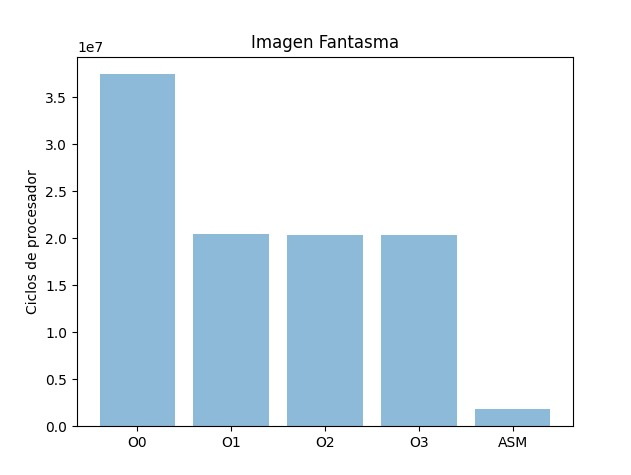
\includegraphics[width=0.5\linewidth]{img/ImagenFantasma.jpeg}\hfil
        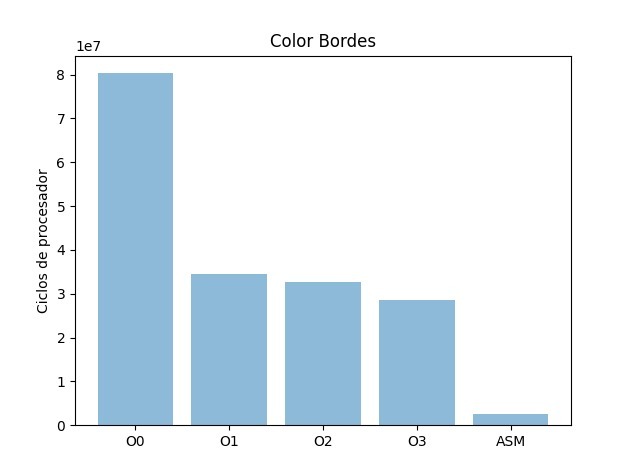
\includegraphics[width=0.5\linewidth]{img/ColorBordes.jpeg}\par\medskip
        \caption{Comparación de promedio de rendimiento para Imagen Fantasma entre ASM y distintas optimizaciones de C}
        \caption{Comparación de promedio de rendimiento para Color Bordes entre ASM y distintas optimizaciones de C}
    \end{figure*}
    
    \begin{figure*}[h]
    \centering
    \begin{tabular}{cc}
        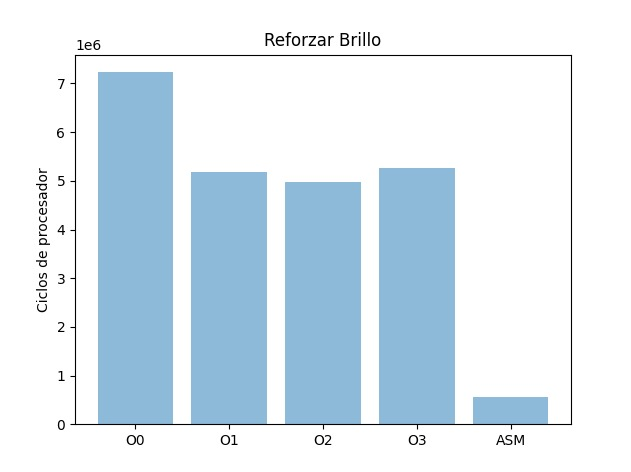
\includegraphics[width=0.5\linewidth]{img/ReforzarBrillo.jpeg}&
    \end{tabular}
    \caption{Comparación de promedio de rendimiento para Reforzar Brillo entre ASM y distintas optimizaciones de C}
\end{figure*}

\par Estas últimas figuras miden el promedio de ciclos de código, donde se excluyeron de la población muestral todas aquellas muestras que se encuentren 2 veces por encima de la desviación estándar.
Estas mediciones fueron hechas con una amplia variedad de imágenes de distintos tamaños y como se puede apreciar, la diferencia de rendimiento entre las implementaciones en ASM es superior
a cualquier optimización de C.

\par Al usar imágenes de distintos tamaños para medir el rendimiento, surgió la pregunta de si el mismo afectaba a la performance de los algoritmos (relativa entre estos), tanto en C como en ASM.
Para esto se escogió un subconjunto de estas imágenes, las cuales fueron reconvertidas para tener los siguientes tamaños: 128x64, 256x128, 512x256 y 1024x512.


\begin{figure*}[h]
    \centering
        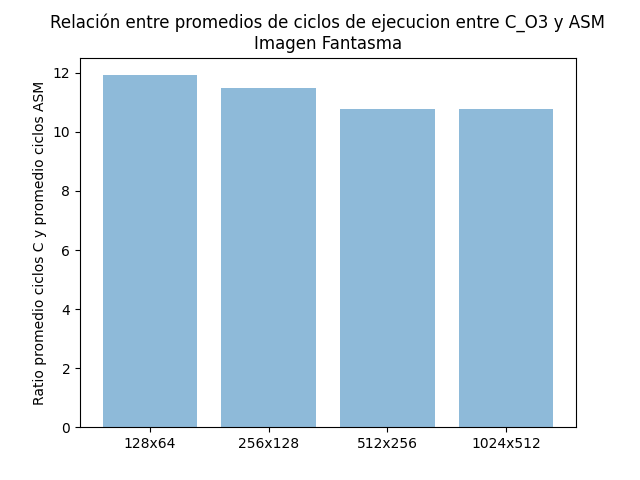
\includegraphics[width=0.5\linewidth]{img/RelacionASMCImagenFantasma.png}\hfil
        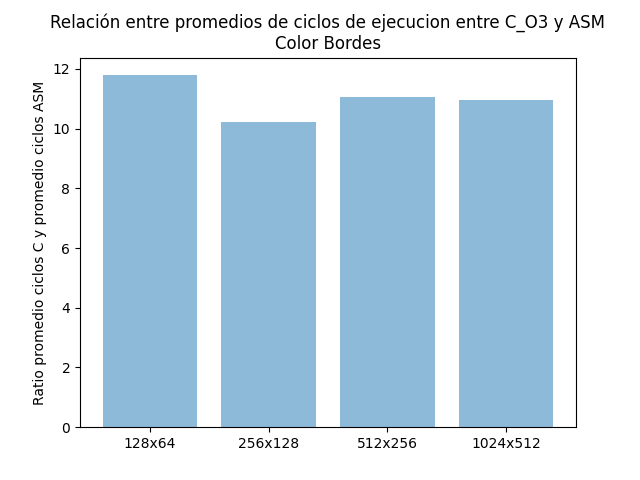
\includegraphics[width=0.5\linewidth]{img/RelacionASMCColorBordes.png}\par\medskip
        \caption{Ratio entre promedios de rendimiento para Imagen Fantasma entre ASM y C_O3 con distintos tamaños de imagenes}
        \caption{Ratio entre promedios de rendimiento para Color Bordes entre ASM y C_O3 con distintos tamaños de imagenes}
    \end{figure*}
    
    \begin{figure*}[h]
    \centering
    \begin{tabular}{cc}
        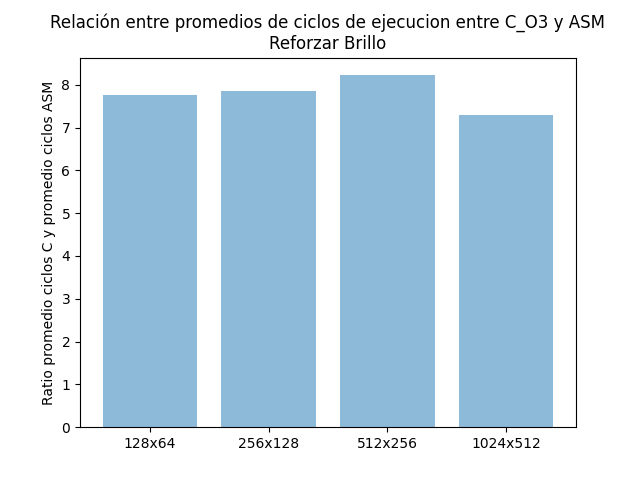
\includegraphics[width=0.5\linewidth]{img/RelacionASMCReforzarBrillo.png}&
    \end{tabular}
    \caption{Ratio entre promedios de rendimiento para Reforzar Brillo entre ASM y C_O3 con distintos tamaños de imagenes}
\end{figure*}
\par Utilizando el mismo método de cálculo de promedios con este nuevo conjunto de imágenes se ve que se mantiene constante el ratio de ciclos en C / ciclos en ASM, lo cual asegura que llevar a cabo 
la comparación ASM vs. C utilizando distintos tamaños de imagen no afecta qué implementación resulta ser la mejor.

\section{Experimentación}
\subsection{Experimento 1}
\subsubsection{Descripción}

\par Se realizaron dos implementaciones alternativas de Imagen Fantasma.
\par Una, en lugar de multiplicar por 0.9, multiplica por 1 (no hace nada).
\par La otra multiplica por 7/8 (0,875) utilizando operaciones de multiplicación de enteros SIMD y shifts en SIMD. A continuación, el código de la misma:

\begin{codesnippet}
    \begin{verbatim}
movdqu xmm1, [rdi + rax]       ; xmm0 = primeros 4 pixeles a partir de i, j


pmovzxbw xmm0, xmm1            ; xmm0 = [2do pixel | 1er pixel]
psrldq xmm1, 8
pmovzxbw xmm1, xmm1            ; xmm1 = [4to pixel | 3er pixel]


movdqu xmm5, xmm0              
; xmm5 = [ a2 | b2 | g2 | r2 | a1 | b1 | g1 | r1 ]
pmulhw xmm5, xmm9              ; xmm5 = 
[ hi(8*a2) | hi(7*b2) | hi(7*g2) | hi(7*r2) | hi(8*a1) | hi(7*b1) | hi(7*g1) | hi(7*r1) ]
pmullw xmm0, xmm9              ; xmm0 = 
[ low(8*a2) | low(7*b2) | low(7*g2) | low(7*r2) | low(8*a1) | low(7*b1) | low(7*g1) | low(7*r1) ]
movdqa xmm6, xmm0              ; xmm6 = 
[ low(8*a2) | low(7*b2) | low(7*g2) | low(7*r2) | low(8*a1) | low(7*b1) | low(7*g1) | low(7*r1) ]
punpcklwd xmm0, xmm5           ; xmm0 = [ 8*a1 | 7*b1 | 7*g1 | 7*r1 ]
punpckhwd xmm6, xmm5           ; xmm6 = [ 8*a2 | 7*b2 | 7*g2 | 7*r2 ]
psrlw xmm0, 3                  ; xmm0 = [ a1 | 7/8*b1 | 7/8*g1 | 7/8*r1 ]
psrlw xmm6, 3                  ; xmm6 = [ a2 | 7/8*b2 | 7/8*g2 | 7/8*r2 ]
packusdw xmm0, xmm6            ; xmm0 = [ 2do pixel | 1er pixel ]

movdqu xmm5, xmm1              ; xmm5 = [ a4 | b4 | g4 | r4 | a3 | b3 | g3 | r3 ]
pmulhw xmm5, xmm9              ; xmm5 = 
[ hi(8*a4) | hi(7*b4) | hi(7*g4) | hi(7*r4) | hi(8*a3) | hi(7*b3) | hi(7*g3) | hi(7*r3) ]
pmullw xmm1, xmm9              ; xmm1 = 
[ low(8*a4) | low(7*b4) | low(7*g4) | low(7*r4) | low(8*a3) | low(7*b3) | low(7*g3) | low(7*r3) ]
movdqa xmm6, xmm1              ; xmm6 = 
[ low(8*a4) | low(7*b4) | low(7*g4) | low(7*r4) | low(8*a3) | low(7*b3) | low(7*g3) | low(7*r3) ]

punpcklwd xmm1, xmm5           ; xmm1 = [ 8*a3 | 7*b3 | 7*g3 | 7*r3 ]
punpckhwd xmm6, xmm5           ; xmm6 = [ 8*a4 | 7*b4 | 7*g4 | 7*r4 ]
psrlw xmm1, 3                  ; xmm1 = [ a3 | 7/8*b3 | 7/8*g3 | 7/8*r3 ]
psrlw xmm6, 3                  ; xmm6 = [ a4 | 7/8*b4 | 7/8*g4 | 7/8*r4 ]
packusdw xmm1, xmm6            ; xmm1 = [ 4to pixel | 3er pixel ]

packuswb xmm0, xmm1            ; xmm0 = [ 4to pixel | 3er pixel | 2do pixel | 1er pixel ]
	\end{verbatim}
\end{codesnippet}




\subsubsection{Pregunta a responder}
\par ¿Cuánta precisión perdemos en el filtro si reemplazamos las operaciones con floats por operaciones con enteros que aproximen multiplicar por 0.9?
¿Cuánta performance se gana? ¿Vale la pena?


\subsubsection{Hipótesis del grupo}
\par En cuanto a performance, se espera que la implementación que multiplica por 1 sea la más veloz con una diferencia notable y que la otra alternativa
sea la segunda más rápida, dejando última a la implementación original.
Por otro lado, en cuanto a la precisión, observando los factores que usamos en los algoritmos, es evidente que la implementación original será la mejor,
dejando atrás a la segunda alternativa y luego a la primera.


\subsubsection{Análisis de los resultados y conclusiones}
\par Para constrastar nuestra hipotesis realizamos dos mediciones distintas. Una, sobre el error existente al utilizar las dos alternativas propuestas contra la original. Luego 
medimos la performance entre las tres implementaciones. En los siguientes gráficos se pueden apreciar los resultados obtenidos.

\begin{figure*}[h]
    \centering
        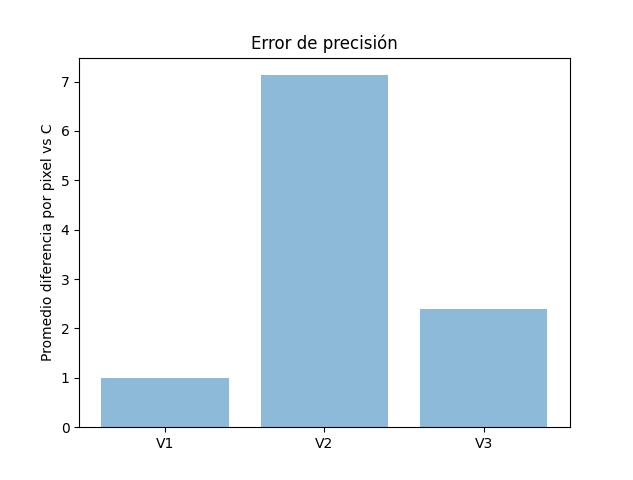
\includegraphics[width=0.5\linewidth]{img/ComparacionErrorExperimentoPato.png}\hfil
        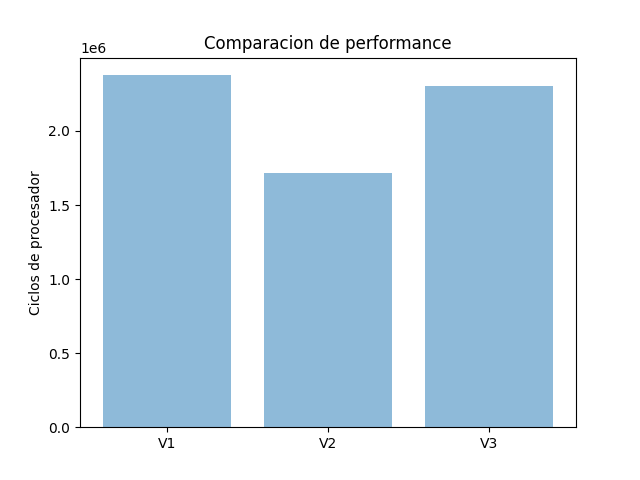
\includegraphics[width=0.5\linewidth]{img/ComparacionPerformanceExperimentoPato.png}\par\medskip
        \caption{Comparación del error entre la implementación original y las dos alternativas}
        \caption{Comparación de performance entre las implementaciones}
\end{figure*}

\par Como se esperaba, la primer alternativa, es sensiblemente más performante que las otras dos. Esto significa que podría ser una opción interesante si se
necesita aplicar el filtro en tiempo real y no se requiere mucha fidelidad. Sin embargo no se notó una diferencia apreciable entre la
implementación original y la segunda alternativa. Esto puede deberse a que contiene múltiples operaciones de pack, unpack, y mov.
\par Por último, la precisión de la segunda alternativa es similar a la de la implementación original, puesto que 7/8 es una aproximación decente de 0.9,
mientras que la primer alternativa es considerablemente peor. Vale la pena notar que la diferencia en las imágenes resultantes de la implementación original y la que tiene peor precisión es altamente
despreciable a simple vista.

\subsection{Experimento 2}
\subsubsection{Descripción}

\par Se corrió la implementación en C del filtro Reforzar Brillo para imágenes del mismo tamaño con los siguientes parámetros: 
\begin{itemize}
	\item un umbral superior de -1, que fuerza en cada iteración a que se entre al primer \texttt{if} y una imagen en negro que provoca siempre el mismo comportamiento en la función saturación
	\item un umbral inferior de 151 y uno superior de 150 que fuerza en cada iteración a que se entre al primer o al segundo \texttt{if}
\end{itemize}
\par La motivación de estos casos era, en primer lugar, predeterminar qué saltos tomará el programa, mientas que en el segundo caso se buscó
maximizar la cantidad de saltos distintos.

\subsubsection{Pregunta a responder}
\par ¿Qué ocurre cuando en el posible flujo del código se toma siempre el mismo camino? ¿Y cuando (a priori) son equiprobables distintos branches? ¿Hay algún mecanismo de predicción de 
saltos que entre en juego? Si lo hay, ¿provoca éste cambios significativos en la performance?

\subsubsection{Hipótesis del grupo}
\par La hipótesis formulada afirma que el mecanismo de predicción de saltos presente en todos los procesadores modernos, sean cuales sean los detalles de su funcionamiento, deberá optimizar 
de alguna manera el caso donde siempre se toma el mismo salto o branch, mientras que en el segundo caso, al ser más impredescible (a menos que se trate de una imagen con todos los píxeles iguales 
o donde todos los píxeles mantienen la misma relación de orden con los umbrales, que no es el caso de este experimento) se espera que haya peor performance del filtro.
Esto se debe a que el procesador tiene más probabilidades de predecir el branch equivocado, y entrarán en juego las penalizaciones por hacer una predicción errónea.

\subsubsection{Análisis de los resultados y conclusiones}
\begin{figure*}[h]
    \centering
        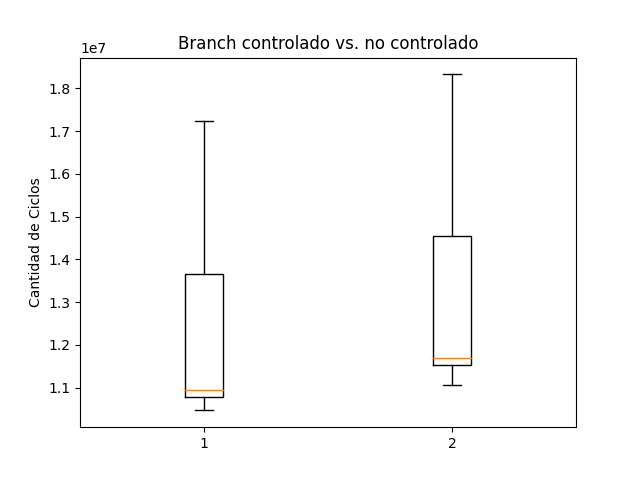
\includegraphics[width=0.5\linewidth]{img/BranchControladoVsNOControlado.jpeg}\hfil
        \caption{Comparación de performance imagen negra vs. imagen normal}
\end{figure*}
\par Se puede observar en la última figura que el rendimiento del primer caso es notablemente mejor que el del segundo. Es evidente que existe una diferencia en el comportamiento del procesador
producto de la imposibilidad de predecir correctamente el camino del segundo caso.


\section{Conclusión}
Como conclusión del informe, logramos crear y utilizar este básico sistema operativo que nos ayudó a aprender sobre los fundamentos de System Programming.
Entendimos lo que conlleva desarrollar sistemas operativos modernos, mucho más complejos y en muchas ocaciones utilizando otros mecanismos que difieren en gran medida de lo implementado en este Trabajo Práctico.



\end{document}

